\chapter{Rencana Pengembangan Milestone 2}
\label{chap:rencana_m2}

Diagram operasional Milestone 1 dimuat bersama pembahasannya pada Bab 2 serta bagian P1, P3, P4, dan P5. Lampiran ini hanya memuat rancangan pengembangan Milestone 2, bukan bukti fitur yang telah berjalan. Sumber kanonis tersedia di \path{docs/diagrams/}.

\section{Scale-Out Layanan}
Gambar~\ref{fig:rencana_scaleout} membandingkan baseline satu instance pada Milestone 1 dengan rencana penambahan replika, load balancer, cache, dan kapasitas broker pada Milestone 2.
\begin{figure}[H]
    \centering
    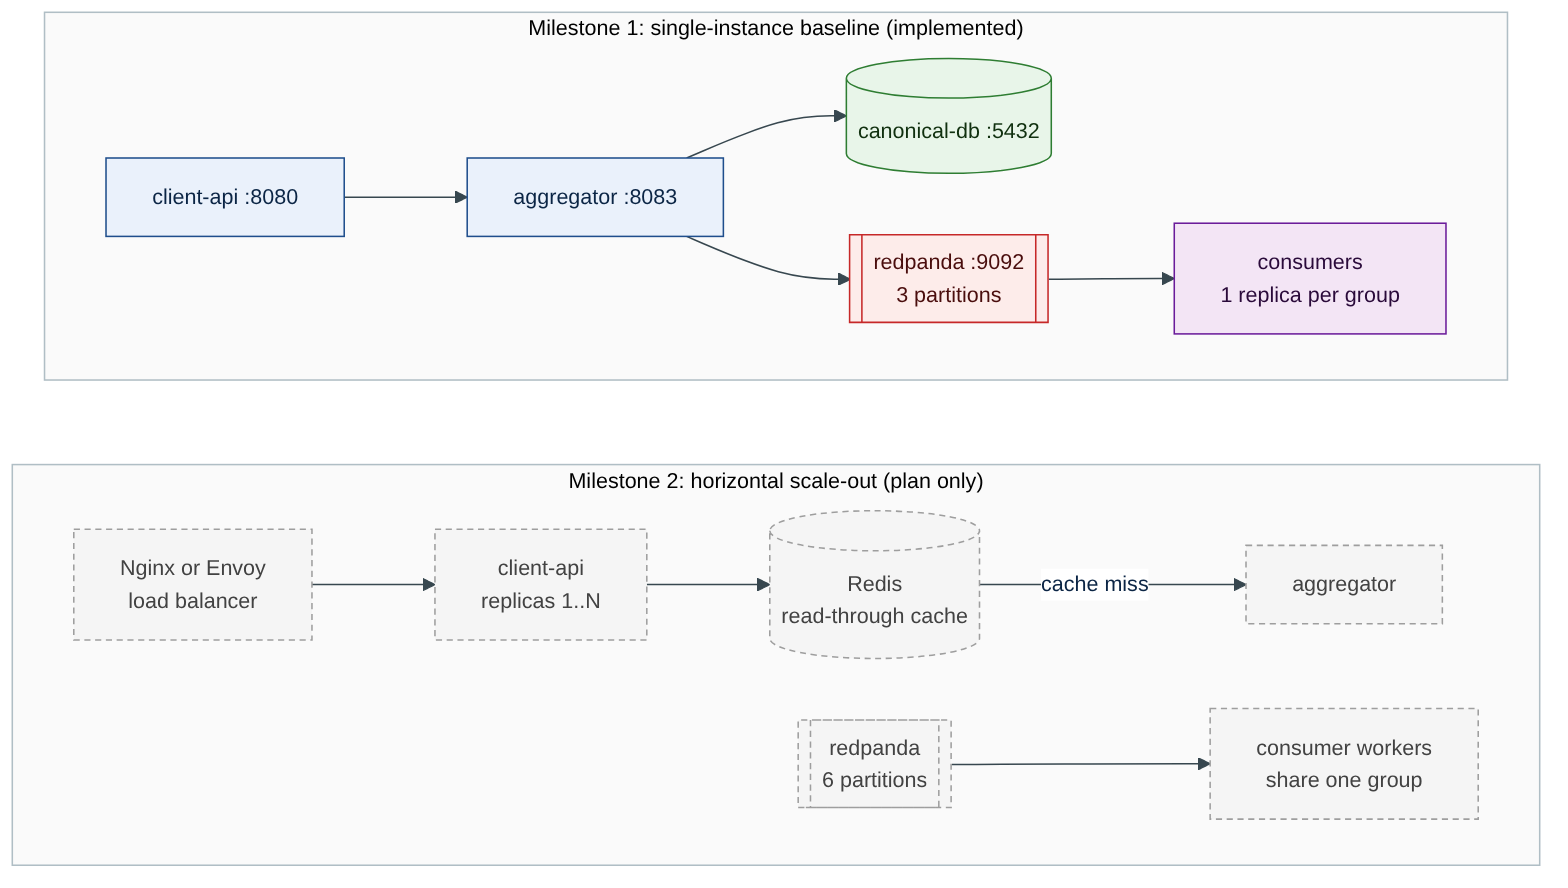
\includegraphics[width=\textwidth,height=0.60\textheight,keepaspectratio]{../diagrams/rendered/adr005-scaleout.png}
    \caption[Rencana scale-out Milestone 2]{Baseline Milestone 1 dan rencana scale-out Milestone 2.}
    \label{fig:rencana_scaleout}
\end{figure}

\clearpage
\section{Circuit Breaker}
Gambar~\ref{fig:rencana_breaker} menunjukkan rencana transisi dari \textit{closed} ke \textit{open} setelah kegagalan berulang, kemudian ke \textit{half-open} untuk menguji pemulihan layanan. Mekanisme ini belum menjadi bagian dari implementasi Milestone 1.
\begin{figure}[H]
    \centering
    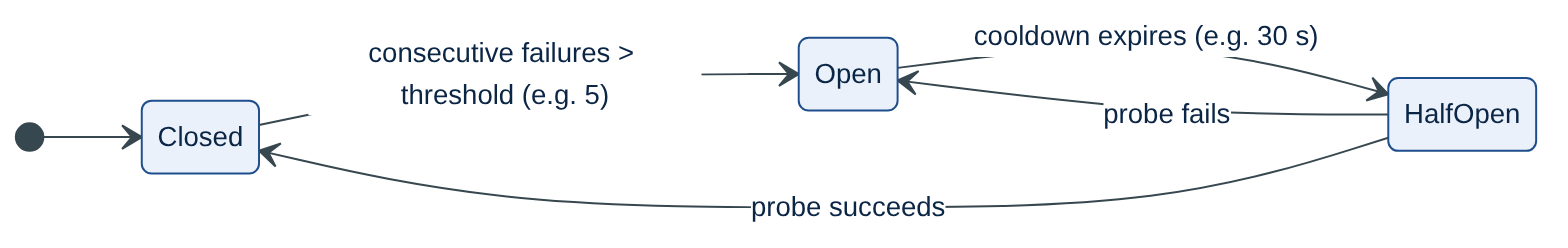
\includegraphics[width=\textwidth,height=0.55\textheight,keepaspectratio]{../diagrams/rendered/adr005-breaker.png}
    \caption[Rencana circuit breaker Milestone 2]{Rencana transisi keadaan circuit breaker untuk Milestone 2.}
    \label{fig:rencana_breaker}
\end{figure}
